% $Id$

Although the upper limit that we have placed on the rate of binary black hole
MACHO inspirals in the galaxy is lower than the upper bound of predicted
rates, the LIGO interferometers were not at design sensitivity when the S2
data was taken. At present, the sensitivity of the instruments are
significantly better than during S2 as can be seen from figure~\ref{f:s3strain}
and progress on reducing noise in the interferometers continues apace.  In
addition to the increased sensitivity making a larger volume of the Universe
accessible to searches for binary inspirals, the amount of data available is
also increasing as the interferometers become more stable.

These improvements in the instruments greatly increase the chance of
detecting gravitational waves from binary inspirals. If the rates of binary
black hole MACHO coalescence are truly as high as predicted then initial LIGO
would stand an excellent chance of detecting an inspiral. The first detection
of gravitational waves will be a major scientific breakthrough and if the
detection came from a binary black hole MACHOs, there would be an enormous
amount of scientific information available. The length of the binary black
hole MACHO signals will allow extremely accurate parameter estimation and
tests of post-Newtonian theory. For systems with total mass greater than $\sim
0.64\,\mathrm{M}_\odot$ LIGO will be sensitive to the coalescence of the
binary and we will be able to study the strong gravitational field effects
when two binary black holes merge. When this is coupled with the accurate
parameter estimation available from the earlier part of the inspiral, binary
black hole MACHOs could be an excellent laboratory for General Relativity.

A detection would also impact the studies of halo dark matter and early
universe physics, providing a MACHO component to the halo and suggesting that
primordial black holes do form in the early universe.

In the absence of detection, the improvements in detector sensitivity will
dramatically improve the upper limits placed on the rate of binary black hole
MACHO inspirals. Once these rates are below the predicted rates, we may begin
to use observation from gravitational wave interferometers to constrain the
fraction of galactic halos in the form of primordial black hole MACHOs. While
this may not be as significant as a detection, it will still be of interest to
the astrophysical community.

\newpage 

\begin{figure}[p]
\label{f:s3strain}
\vspace{5pt}
\begin{center}
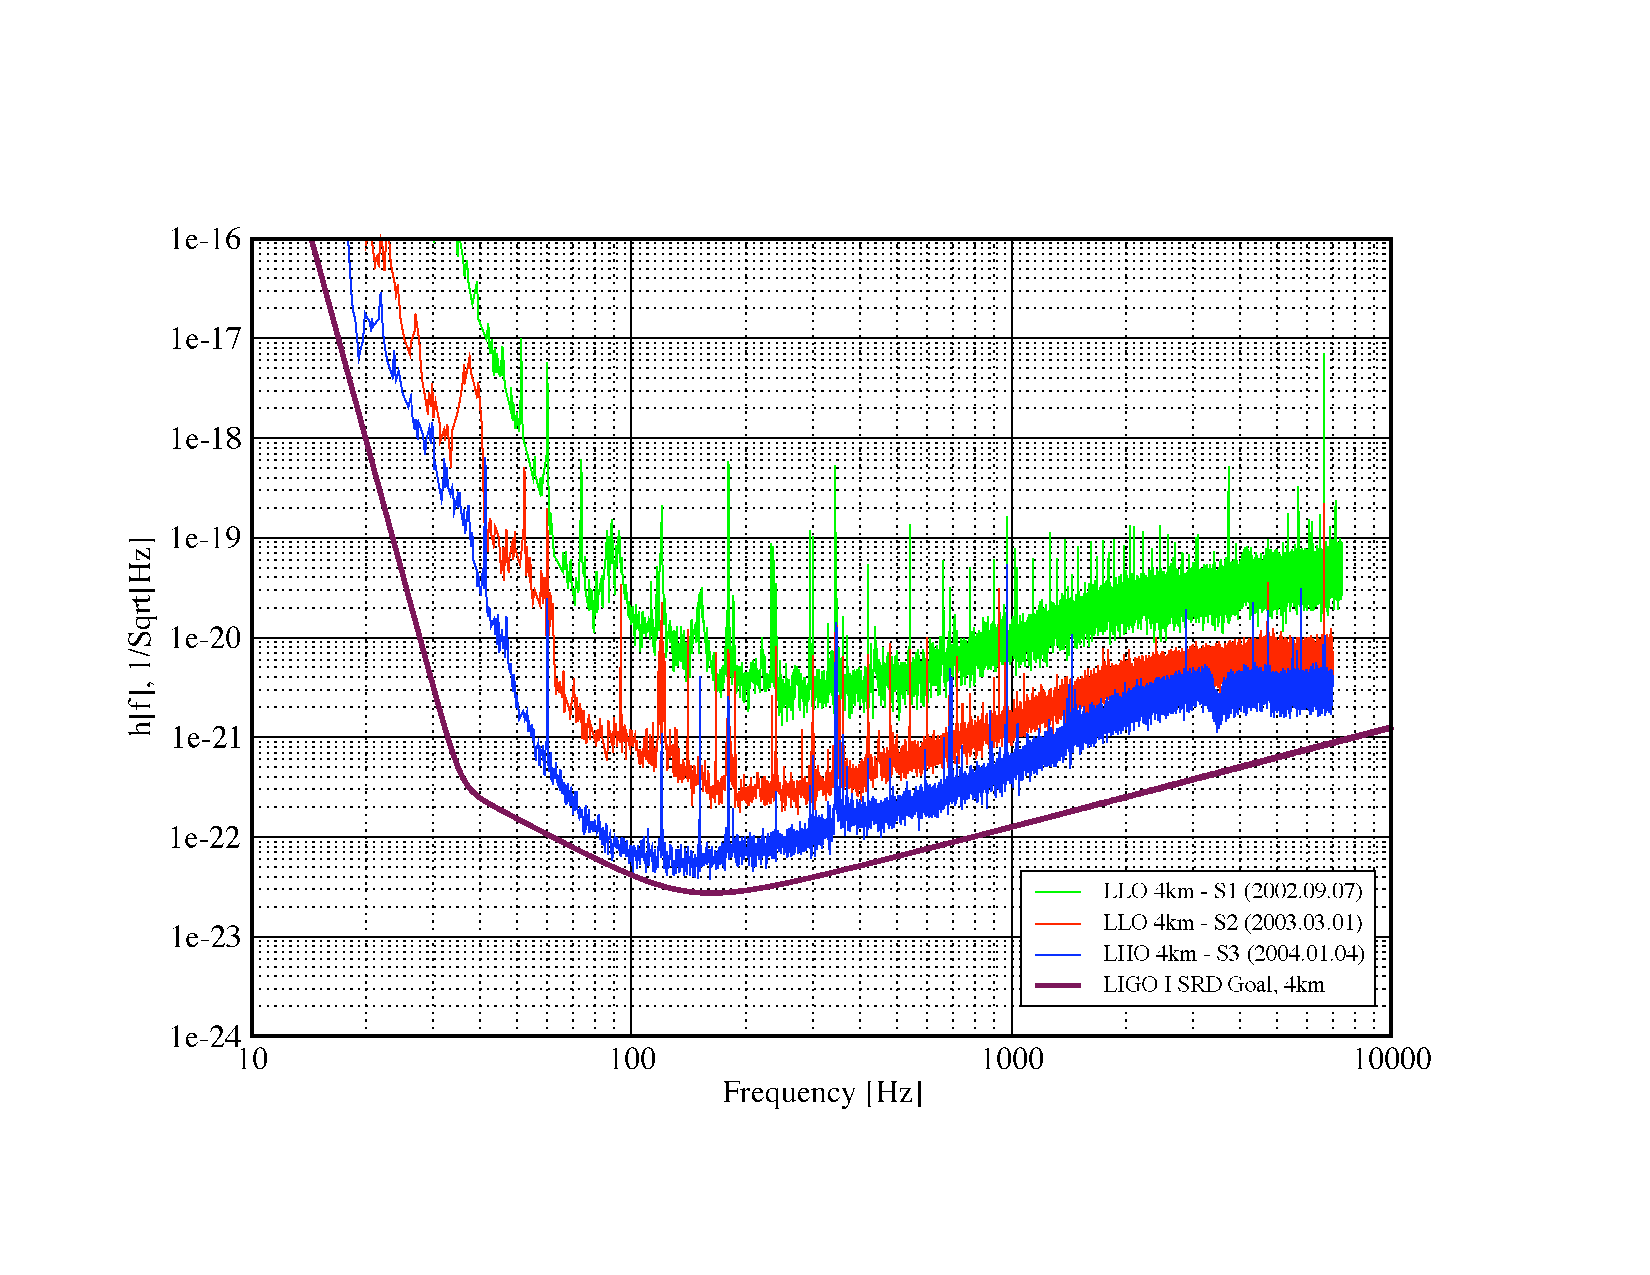
\includegraphics[width=\textwidth]{figures/conclusion/s3strain}
\end{center}
\caption[Comparison of Best LIGO Interferometer Sensitivity]{%
Comparison of the best sensitivities of the LIGO interferometers between
science runs. The solid curve shows the design sensitivity for the $4$~km
interferometers: the LHO $4$~km is only a factor of $\sim 2$ away from design
at $100$~Hz during S3.
}
\end{figure}

